%%%%%%%%%%%%%%%%%%%%%%%%%%%%%%%%%%%%%%%%%%%%%%%%%%%%%%%%%%%%%%%%%%%%%%%%%%%%%%%%%%%%%%%%%%%%%%%%%%%%%%%%%%%%%%%%%%%%%%%%%%%%%%%%%%%%%%%%%%%%%%%%%%%%%%%%%%%
% This is just an example/guide for you to refer to when producing your supplementary material for your Frontiers article.                                 %
%%%%%%%%%%%%%%%%%%%%%%%%%%%%%%%%%%%%%%%%%%%%%%%%%%%%%%%%%%%%%%%%%%%%%%%%%%%%%%%%%%%%%%%%%%%%%%%%%%%%%%%%%%%%%%%%%%%%%%%%%%%%%%%%%%%%%%%%%%%%%%%%%%%%%%%%%%%

%%% Version 2.5 Generated 2018/06/15 %%%
%%% You will need to have the following packages installed: datetime, fmtcount, etoolbox, fcprefix, which are normally inlcuded in WinEdt. %%%
%%% In http://www.ctan.org/ you can find the packages and how to install them, if necessary. %%%
%%%  NB logo1.jpg is required in the path in order to correctly compile front page header %%%

\documentclass[utf8]{frontiers_suppmat} % for all articles
\usepackage{url,hyperref,lineno,microtype}
\usepackage[onehalfspacing]{setspace}
\usepackage{amsmath}
\usepackage{graphicx}
\usepackage{listings}
\usepackage{ textcomp }
\usepackage{pbox}
\usepackage{xr}
\externaldocument{frontiers}

\lstdefinestyle{myCustomStyle}{
  stepnumber=1,
  numbersep=10pt,
  tabsize=3,
  showspaces=false,
  showstringspaces=false,
  breaklines=true,
  postbreak=\mbox{\textcolor{red}{$\hookrightarrow$}\space}
}

\lstset{
   basicstyle=\fontsize{8}{10}\selectfont\ttfamily,style=myCustomStyle
}

\makeatletter
\newcommand*{\addFileDependency}[1]{% argument=file name and extension
  \typeout{(#1)}
  \@addtofilelist{#1}
  \IfFileExists{#1}{}{\typeout{No file #1.}}
}
\makeatother

\newcommand*{\myexternaldocument}[1]{%
    \externaldocument{#1}%
    \addFileDependency{#1.tex}%
    \addFileDependency{#1.aux}%
}

\myexternaldocument{frontiers}


% Leave a blank line between paragraphs instead of using \\

\begin{document}
\onecolumn
\firstpage{1}

\title[Supplementary Material]{{\helveticaitalic{Supplementary Material}}}


\maketitle

\section {MIIND Directory Structure}
\label{directorystructure}

\begin{lstlisting}
MIIND_HOME/
    apps/
    cmake-modules/
    doc/
    examples/
    images/
    libs/
    package/
    Publication/
    python/
    CMakeLists.txt
\end{lstlisting}

The top level directory structure of the MIIND code base. $libs$ holds the main library code. $apps$ contains the ancillary executables such as MatrixGenerator and Projection as well as various tests and C++ examples. $python$ contains the full MIIND Python API including the command line interface. $examples$ contains a a selection of example simulations which can be run using the $miindio.py$ command line interface. $package$ contains the files necessary to generate a debian package and docker image of MIIND. \textit{CMakeLists.txt} is the highest level cmake file for building MIIND, supported by additional scripts in \textit{cmake-modules}. Finally, $doc$, $images$, and $Publication$ hold files required to building the doxygen documentation.

\section{Description of the architecture and functionality}
The main architectural concerns in MIIND relate to the two C++ libraries, MPILib and TwoDLib. MPILib is responsible for instantiating and running the simulation, leveraging the use of Boost for MPI parallelisation. TwoDLib contains an implementation of the two dimensional population density technique and is also responsible for generating the transition matrix. Of the remaining libraries, GeomLib contains a population density technique implementation of neuron models with one time dependent variable, although it is also possible and indeed preferable to use the TwoDLib code for one dimensional models. EPFLLib and NumtoolsLib contain helper classes and type definitions. Fig. \ref{fig:uml} shows a reduced UML diagram of the MIIND C++ architecture.\\

\subsection{MPILib}

The MPINetwork class in MPILib represents a simulation as a whole and is instantiated in the main method of each auto-generated simulation executable. MPINetwork exposes member functions for building a network of nodes where each node is an instance of a neuron population which can be connected together so that the output activity from one population is input to another. The class also contains all of the simulation parameters such as the simulation length and time step. Finally, the MPINetwork class exposes a function to run the simulation in its entirety or take a single evolve step for use in an external control loop.\\

Each node in the population network is represented by an instance of the MPINode class. A node has a name and an ID which is used to uniquely identify it in the simulation. A node also contains an implementation of an AlgorithmInterface which implements the integration technique required for this population. The $NodeType$ describes whether a population should be thought of as excitatory or inhibitory. MIIND performs a validation check that the synaptic efficacy from a node is positive or negative respectively. There is also a ``Neutral'' node type in case the population should be considered heterogeneous and can therefore produce both positive and negative efficacies. During each iteration, each node is responsible for consolidating the activity of all input connections, calling the integration step in the AlgorithmInterface implementation, and reporting the density and output activity (the average firing rate).\\
In MPILib, a number of implementations of AlgorithmInterface are defined which can be instantiated in a node and are responsible for the lion's share of the computation in MIIND as this is where the integration of the model is performed. The interface is extremely simple, providing a function to set parameters, an optional function for a preamble before each iteration, and the $evolveNodeState$ function to be called for every time step. MIIND's two dimensional population density technique is an implementation of this interface but is defined in TwoDLib. MPILib has a number of other implementations.

\begin{itemize}
\item A rate algorithm which takes no input and trivially produces a constant firing rate
\item A ``rate functor'' algorithm which takes a function as an argument which will produce a rate based on the time or other parameters
\item A delay algorithm which delays output of its input rate by a certain time interval
\item A Wilson-Cowan algorithm which can implement a number of variations of the Wilson-Cowan population model \citep{wilson1972excitatory}
\end{itemize}

\subsection{MPI Implementation}
MIIND supports parallelisation using MPI by sharing out the responsibility for evolving each population (each node in the network) across the available processes. Nodes are assigned in a round robin fashion although MIIND can support other load balancing policies if required. The integration of each node is self contained within each process and all processes synchronise at the end of each iteration step. At this point, each node must receive the computed activity value from all connected nodes which input to it. If the activities have been calculated in other processes, this will require an MPI message to be sent from the producing node and received by the connected node. The utility class, MPIProxy wraps the Boost MPI functionality to set up new processes, send and receive messages, and synchronise. The CircularDistribution utility class implements the round robin load balancing policy and provides a function for identifying the process responsible for a given node. \\
While the overhead of message passing and initial set up limit the benefits of MPI with only a small number of nodes, there is a marked improvement in efficiency with more than four or five populations.\\

\subsection{TwoDLib}
As with the population models in MPILib, MIIND's geometric population density technique is an implementation of the AlgorithmInterface named MeshAlgorithm. MeshAlgorithm is supported by two further classes. Ode2DSystem performs the pointer update for quickly solving the deterministic dynamics of the population, as well as transferring probability mass according to the reset and reversal mappings. MasterOdeint is responsible for solving the Poisson master equation using the transition matrix. For each iteration, the function $evolveNodeState$ is called which performs the four main steps in the population density algorithm. \\
First, all cells in the mesh are shifted one position along their strips by the $Evolve$ function in Ode2DSystem. Mass in the last cell of a strip is shifted back to the first cell of the strip. The first cell is guaranteed to be empty as any mass which was there would already have been shifted to the second cell. \\

The second step is for Ode2DSystem to perform any reversal remappings. It is often the case that we do not want mass to shift back to the beginning of a strip. This would likely represent a completely unrealistic jump of a neuron's state that is not permitted by the neuron model. Because strips are generated by following the dynamics of the neuron model, often strips will approach a stable point in the state space. As the neuron's state approaches this point, the size of each consecutive cell in the strip will become infinitesimally small. To avoid this, the strip is curtailed a certain distance before reaching the stable point and the small area around the stable point is covered with a separate strip consisting of a single cell. As predicted by the model, mass accumulates in the single cell and does not move unless incoming spikes push it out. To facilitate mass moving from the end of a strip into a stationary cell, a reversal remapping is performed to take the mass from the first cell of the strip and place it in the stationary cell. The reason mass is taken from the first cell is that that mass was in the last cell of the strip before being moved during the previous $Evolve$ step. There are other scenarios where we wish to dictate where mass moves after reaching the end of a strip. For example, a limit cycle attractor may be covered by a single strip (this is actually a case where we do want mass to be cycled back from the last cell to the first). The last cells of strips approaching this limit cycle will need reversal mapping to the correct cell on the attractor strip.\\

The third step calls on the MasterOdeint class to solve the master equation for the incoming Poisson spike rates from every incident node. MasterOdeint requires the current state of the probability mass distribution across the mesh, that is, the values of each cell in the mesh. It also requires the transition matrix. After a single spike, the mass in a cell is likely to have spread across only a few other cells. The transition matrix is therefore sparse and is stored as a compressed sparse row (CSR) matrix. The change to the mass distribution, $\rho$, is defined as \\

$d\rho/dt = \lambda * M * \rho \\$

The boost numeric library is used to integrate $d\rho/dt$. The solution to this equation describes the spread of the population due to Poisson spikes. This `Master process' step is where the majority of time is taken computationally. However, OpenMP is available in MIIND to parallelise the matrix multiplication. If multiple cores are available, the OpenMP implementation significantly improves performance of the master process step.\\
The final step in the $evolveNodeState$ function is to perform any ``reset'' mappings. Similar to the reversal mappings, this step is useful for neuron models, such as leaky integrate and fire, which contain an instruction to reset one or more variables to a different value upon reaching a threshold. Leaky integrate and fire requires the membrane potential to be reset to a specified value when it reaches threshold. During the generation of the transition matrix, cells which lie across a user defined threshold value are identified as the threshold cell group and sorted in ascending order along the threshold line which extends through the second dimension. The same sorting is performed for the group of cells which lie along a user defined reset value. For each cell in the threshold group, the centroid of the cell is shifted back to the reset value and optionally shifted up or down along the second dimension. The AdExp model is an example where, at the threshold, a neuron is reset to a lower membrane potential and the second additive variable is increased slightly. The mass that is in the threshold cell is shared out between the two reset cells which sit above and below the translated centroid proportional to their distances. This proportionality is calculated during the matrix generation preprocessing step. At run time, in the $evolveNodeState$ function, the mass that sits in each threshold cell is shared among its two reset cells. As passing the threshold and being reset represents a neuron firing, all mass which was reset from all of the threshold cells is summed and divided by the simulation time step. This value is the average firing rate of the population for this iteration.\\

\subsection{MIIND Library Dependencies}
\label{miinddependencies}
This section lists some of the third party libraries on which MIIND depends and are widely available on multiple platforms. While most are necessary for MIIND to run, some libraries such as ROOT and the CUDA libraries are optional but will limit functionality if unavailable. The full list of dependencies is available in the MIIND code repository.

\subsubsection*{Root (Optional)}
Root \citep{brun1997root} is a library which provides useful data analysis and plotting tools for scientific applications. Because Root is not required for any of the major MIIND functionality, it is an optional dependency and can be disabled when building MIIND using the \textbf{ENABLE\_ROOT} flag. Disabling ROOT removes the ability to use the \textit{\textless SimulationIO\textgreater} block in the XML file for GeomAlgorithm. 

\subsubsection*{Boost}
The basic installation of Boost is a ``header only'' extension of the C++ standard. MIIND uses Boost to support parallel processing tasks such as the MPI functionality and for solving the Poisson master equation. It is also used for timing and other convenience methods. Because MIIND uses Boost for the MPI processing, the pre-built boost-mpi library must be installed before MIIND will function even if MPI is disabled. 

\subsubsection*{CUDA (Optional)}
In order to use the GPGPU implementation of the MIIND population density technique (MeshAlgorithmGroup and GridAlgorithmGroup), the machine running MIIND must have a CUDA enabled graphics card with the requisite CUDA libraries. Set \textbf{ENABLE\_CUDA} in the MIIND installation to use the vectorised (Group) algorithms.

\subsubsection*{MPI (Optional)}
MPI can be enabled in the MIIND installation with \textbf{ENABLE\_MPI}. 

\subsubsection*{OpenMP (Optional)}
OpenMP is another parallel processing solution which runs specified code blocks in parallel across multiple cores. It is recommended that OpenMP is enabled if possible even if the vectorised algorithms are to be used on the GPU. This is because OpenMP is also used to improve the performance of the geometric transition matrix generator. The \textbf{ENABLED\_OPENMP} flag in the MIIND installation can be used to enabled OpenMP.

\section{CUDA Implementation}
\label{cudaimplement}
The MIIND CUDA implementation performs similar steps to the CPU version but relies on a different code path which uses the VectorisedNetwork class to contain a simulation. The main function of the generated .cu file instantiates VectorisedNetwork which is in the MiindLib library. VectorisedNetwork is designed to run a simulation of vectorised population densities only. For each Node defined in the simulation XML, the main class calls addGridNode, addMeshNode or addRateNode depending on the algorithm type. This is a departure from the CPU version which insantiates the algorithms themselves and passes those as parameters to each node.\\
The connections between nodes is defined using the functions addGridConnection, addMeshConnection and addMeshCustomConnection which instantiate an internal class for each connection type required for vectorised simulations.\\
Once all nodes and connections are set up, the initOde2DSystem and setupLoop functions are called which organise the separate mass vectors and transition matrices of the individual nodes into contiguous data structures (Fig. \ref{fig:cudastruct}) ready for parallel processing on the GPU. In initOde2DSystem, the mass vectors of each Grid and Mesh node are concatenated into a single vector, \_vec\_mesh. The reversal and reset mappings for each node and a list of refractive times are also generated. These structures are passed to an instance of CudaOde2DSystemAdapter in the CudaTwoDLib library. The transition matrices for the deterministic dynamics of the grid nodes are concatenated into the \_csrs vector which will hold all transition matrices required for the simulation. In the setupLoop function, \_csrs is further appended with the transition matrices for solving the master equation for each node (both grid and mesh). The \_csrs vector along with total number of connections, timestep and index lists (mapping the network connections to their associated transition matrices) are passed to an instance of CSRAdapter. The two classes CSRAdapter and CudaOde2DSystemAdapter in the CudaTwoDLib library are responsible for making calls to the Cuda functions defined in CudaEuler. The function singleStep in VectorizedNetwork, performs a single step of the simulation in a similar fashion to the CPU version of the code. The following algorithm steps are performed.\\

\subsection{Update the firing rates and Evolve the Deterministic Dynamics}

Each connection has an associated queue of length one or more which allows for transmission delays (implemented in the same way as a refractory period as described in section \ref{miindoverview} of the main text). The first task of singleStep is to pop the firing rate from the end of each queue to be passed to the associated target populations. As with the algorithm in TwoDLib::MeshAlgorithm, the deterministic dynamics of each node is progressed forward by one time step. By calling CudaOde2DSystemAdapter::Evolve(), the mapping of each cell in each Mesh Node, defined in TwoDLib::Ode2DSystemGroup, is shifted by one along each strip. This mapping is then passed to the graphics card. CudaOde2DSystemAdapter::RemapReversal() calls a serial cuda function defined in CudaEuler and transfers mass according to the reversal mapping which was loaded onto the card earlier. \\
In order to evolve the deterministic dynamics of the grid nodes, the Grid Node Transform Matrices in the \_csrs vector must be applied once to their respective mass vectors. \\

\subsection{Performing the Reset Remapping}

In both the Grid and Mesh nodes, cells which lie on the membrane potential threshold are identified and, during each time step, mass in these cells must be moved to cells which lie on the reset potential. However, if the underlying neuron model includes a refractory period, this must also be taken into account when resetting the mass. The function, CudaOde2DSystemAdapter::RedistributeProbability(), performs the full process on the graphics card. Fig. \ref{fig:cudareset} shows the memory structure required to perform the reset functionality on the card. \_res\_to\_mass stores the mass in cells at the threshold in the current time step. \_res\_sum stores the result of summing \_res\_to\_mass and is extracted to the CPU to produce the current average firing rate. The \_refractory\_mass block holds the refractory queue for each threshold cell. Each refractory queue has length equal to the number of time steps in the refractory period plus one. 

In CudaOde2DSystemAdapter::RedistributeProbability(), first the two blocks, \_res\_to\_mass and \_res\_sum, are zeroed. Next, each value in the refractory queues of \_refractory\_mass is shifted to the right towards the end of the queue, leaving an empty space at the beginning. CudaEuler::MapResetToRefractory() moves the mass in each threshold cell to the now empty first position in its respective refractory queue. The threshold cell mass values are also copied to \_res\_to\_mass for summing later. The additional position in each refractory queue is required in the case where the refractory period is not an integer multiple of the time step. In this case, only a proportion of the mass at the end of the queue is passed to the required reset cell. The remaining mass is then shifted to the additional cell and passed to the reset cell during the next iteration. Therefore, in each iteration, a reset cell receives a proportion of mass from the end cell of the queue and $1 - proportion$ of the mass from the additional cell. Finally, sumReset is called and the result of summing \_res\_to\_mass is passed to \_res\_sum.\\

\subsection{Solve the Master Equation for the Stochastic Noise Process}

For all nodes, using both grid and mesh algorithms, solving the spread of mass across the state space due to incoming Poisson distributed spikes is achieved through multiple applications of the associated transition matrices. The mass vector for each of the nodes in \_vec\_mesh are multiplied by each of the transition matrices in \_csrs corresponding to incoming connections.\\
The VectorizedNetwork variable \_master\_steps, which can be set by the user in the XML file, defines how many times the matrix multiplication is performed. \_master\_steps must be large enough to keep the Euler numerical integration stable. The stability is dependent on the input rate of the connection and the size of the transition for each cell (which in turn is dependent on the efficacy and local dynamics of the mesh). \\
For this part of the process, the grid and mesh algorithms only differ in the way that the transition matrices are generated. As discussed, the mesh algorithm $.mat$ files are pre-generated and passed as a static data structure. For the grid algorithm, the transitions matrix can be generated online due to the regularity of the grid cells which allows for more flexibility in their definition.\\

\subsection{Grid Algorithm Specialisations}
\label{gridalgospec}
The regularity of the grid cells in the GridAlgorithm allows MIIND to calculate the transition matrix for solving the Poisson master equation at run time.  When using GridAlgorithms, then, the connections can be somewhat dynamic, for example, depending on the average membrane potential of the In or Out populations. Because the way that the transition matrix is calculated can be very model specific, this must be defined in a C++ extension to the existing code base. However, two model cases are available for use ``as is’’ or as a template. Example simulations of both of these models is available in the model archive in the code repository.\\

\subsubsection{Minimal Motor Neuron}
The minimal motor neuron model by Booth and Rinzel \cite{booth1995minimal} is a two compartment model with a soma and dendrite part. Each part is comprised of a two dimensional dynamical system including a term which integrates the membrane potential from the other compartment. \\

An approximation of a population of these motor neurons can be simulated in MIIND by using the specialised algorithm GridSomaDendriteAlgorithm to simulate the behaviour of a population of somas and a population of dendrites. This is clearly different to a population of individually coupled pairs which is why it is an approximation. To account for the term in each of the compartments representing the membrane potential of the opposing part, MIIND uses the average membrane potential of each population. Two connections are defined between the GridSomaDendriteAlgorithm populations to pass the shared average membrane potential values. The connections are identified with a type attribute equal to ``SomaDendrite'' and a ``conductance'' which represents the degree of coupling of the two populations as described by \cite{booth1995minimal}. A specialised solver for the Poisson master equation solver, ``MasterGridSomaDendrite'' takes the conductance value of the connection and multiplies this by the difference between the membrane potential of each cell and the average membrane potential of the other population (provided via the connection). The GridSomaDendriteAlgorithm is currently not available for use with the GPGPU.\\
\\
\subsubsection{2D Epileptor}
The 2D Epileptor neuron model \citep{proix2014permittivity,proix2017individual} is a reduced version of the full Epileptor model \citep{jirsa2014nature} developed for use with The Virtual Brain for investigating the propagation of epileptic seizures across the whole brain. As with the GridSomaDendriteAlgorithm, the model calls for populations connected using more than just the average firing rate or membrane potential. The efficacies of two Epileptor populations are calculated using the K and tau parameters which must be provided as attributes to connections with type ``epileptor''. How these values are used is described by \cite{proix2014permittivity}. Unlike the GridSomaDendriteAlgorithm, a separate algorithm type is not defined for the Epileptor as the integration of the population is no different to any other grid. The difference is only required at the level of the connections which must be set with the correct attributes.

\section{Generating Marginal Density Plots}
\label{marginalsdensities}
The density files generated by MeshAlgorithm and GridAlgorithm (and variants) can be used to plot both the joint distribution of the two time dependent variables and the marginal densities showing the distribution across each individual dimension. The marginal density is essentially a histogram of the probability mass along each axis of the state space. The required dimension is split into equal-sized bins and, at a given simulation time, the total mass inside each bin is summed. For densities from MeshAlgorithm, mesh cells may span multiple bins so the correct proportion of probability mass in each cell must be attributed to the correct bin. This is also true of the GridAlgorithm although the cells are more regular. In order to calculate the attribution of mass to bins, yet again, the geometric method for generating transition matrices can be used. The area of overlap of a cell with each bin is calculated as described in section \ref{gridgenerate} of the main text and used to define the proportion to be attributed to that bin. The \textit{Projection} program which is a separate executable similar to \textit{GenerateMatrix} implements the algorithm for calculating the transition matrix which is then stored in a $.projection$ file in the working directory of the simulation XML file. The projection file is then used for calculating the specific marginal density for a specific time in the simulation. When the \textbf{plot-marginals} command is called in \textit{miindio.py}, if the projection file does not exist or the mesh has been modified since the projection file was last generated, the \textit{Projection} executable is called first then the specific marginal density can be calculated for the requested time point. As with plotting the full density, the time point parameter passed to \textbf{plot-marginals} must match a density file in the output directory of the simulation which therefore requires that the simulation includes a \textit{\textless Density\textgreater} entry in the \textit{\textless Recording\textgreater} section of the XML for the given population node. In order to plot the marginals of a given node in the simulation, a projection file for the associated model file must have been generated.

\section{Mesh Building tips}
\label{meshtips}
The following are a set of methods to aid in the building of meshes for use with MeshAlgorithm (see Fig. \ref{fig:tips} for illustrations).\\
\subsection{Backwards Integrating}
Many models have a volume of state space where trajectories quickly approach infinity with the expectation that the neuron will be reset above a certain threshold. In these models strips can become extremely shear as one side of the strip increases quicker than the other. All points will also quickly become too high to be represented and the integration of the trajectories will fail. Sometimes it is possible to simply cut short all strips before they reach a certain threshold where these problems occur. However, an alternative is to choose the starting locations of the trajectories at some high value beyond the threshold and backwards integrate.

\subsection{Using Nullclines}
The nullclines of a model can give a good indication of where starting positions should be placed. Where trajectories flow away from a nullcline, starting positions can be chosen just slightly on either side such that strips will travel away. The gap that is left along the nullcline itself is unimportant as the instability on that line would mean that neurons will quickly move to one side or the other. Likewise, where trajectories approach a nullcline, it can be useful to choose starting points on either side and backwards integrate.

\subsection{Strip Stitching}
Strip stitching involves using the reversal mapping to pass mass from the end of one strip to the start of another. this can be useful in a number of situations. For example, if the model to be built has a limit cycle (such as the FitzHugh-Nagumo neuron model), it is often preferable to have a single strip which follows the cycle and have strips which approach the limit cycle but stop short of the cycle strip itself. The reversal mapping can then be used to shift mass form the end each strip to the nearest cell on the cycle strip. This prevents extreme shearing of the cells as they begin to wind around the limit cycle. 
Often there are areas of state space where cells are generally large and regular. Even if these are situated among areas of high cell density (for example, within the bend of a nullcline), it can be beneficial to pick a line or curve of starting points which passes through the area of low density then both forward and backwards integrate from each point. Strip stitching must be employed to attach the two opposing strips together for each of the starting points. 
As with reversal mappings for transferring mass to a stationary cell, the mapping must be defined between the first cell of strip one and the first cell of strip two to account for the shift of mass occurring before the mapping is performed during each time step.

\section{Parameter Sweeps using Variables}
\label{parametersweeps}
As discussed in section \ref{variables} of the main text, the use of Variables in the XML file support convenient methods for performing parameter sweeps. The first method can be used to generate a single executable simulation for each parameter combination required which can then be executed in parallel on high performance systems. As an example, suppose that an experiment is carried out to observe the effect of noise on a population of LIF neurons. As described in section \ref{handlingnoise} of the main text, two quantities can be set to control the mean and variance of the change to the probability density: the input rate and the efficacy. To perform a parameter sweep across these two quantities, the appropriate variables can be declared and added to the XML as in listing \ref{lst:noisevariables}.

\begin{lstlisting}[caption={An abridged version of an XML file with two variables to control the input rate and efficacy of a population of LIF neurons.  }\label{lst:noisevariables}]
...
<Variable Name="RATE">1500.0</Variable>
<Variable Name="EFFICACY">0.01</Variable>
...
<Algorithm type="MeshAlgorithm" name="E" modelfile="lif.model" >
<TimeStep>0.001</TimeStep>
<MatrixFile>lif_0.01_0_0_0_.mat</MatrixFile>
<MatrixFile>lif_0.02_0_0_0_.mat</MatrixFile>
...
<MatrixFile>lif_0.1_0_0_0_.mat</MatrixFile>
</Algorithm>
<Algorithm type="RateFunctor" name="ExcInput">
<expression>RATE</expression>
</Algorithm>
<Nodes>
<Node algorithm="E" name="LIF" type="EXCITATORY_DIRECT" />
<Node algorithm="ExcInput" name="Inp" type="NEUTRAL" />
</Nodes>
<Connections>
<Connection In="Inp" Out="LIF">1 EFF 0</Connection>
</Connections>
<Reporting>
...
\end{lstlisting}

When running miindio.py and calling the sim command, the simulation can be built and run using the default values for RATE and EFFICACY in the Variable definitions. By calling sim with additional parameters setting a name for the simulation and key-value pairs for the two variables, a new XML file will be generated in which the variables have been replaced according to the key-value pairs.

\begin{lstlisting}
> sim lif.xml lif_param_sweep RATE=750.0 EFFICACY=0.02
\end{lstlisting}

The newly generated XML file's name will contain a hashed code which represents the unique combination of key-value pairs so that the experiment can be uniquely identified. All generated simulations will be built into separate output directories under the parent directory named with the given simulation name (lif\_param\_sweep in the example). In the example, as the MeshAlgorithm is used, and the efficacy is controlled by a variable, all transition matrices must have been pre-generated and quoted in the algorithm definition. The process of generating each individual simulation does not need to be performed manually by the CLI. It can be automated using the Python MIIND API. \\

\subsection{Building a Single Python Shared Library to Perform Sweeps}
An alternative to generating multiple executables is to generate a single shared Python library with the requisite constructor parameters. The XML file in listing \ref{lst:noisevariables} can be altered so that the rate is controlled by a Python external connection, and the efficacy remains a variable to be set in the Python script.

\begin{lstlisting}[caption={An abridged version of an XML file to be used to generate a Python shared library with a single variable to control the efficacy.  }\label{lst:noisevariablespython}]
...
<Variable Name="EFFICACY">0.01</Variable>
...
<Algorithm type="MeshAlgorithm" name="E" modelfile="lif.model" >
<TimeStep>0.001</TimeStep>
<MatrixFile>lif_0.01_0_0_0_.mat</MatrixFile>
<MatrixFile>lif_0.02_0_0_0_.mat</MatrixFile>
...
<MatrixFile>lif_0.1_0_0_0_.mat</MatrixFile>
</Algorithm>
<Nodes>
<Node algorithm="E" name="LIF" type="EXCITATORY_DIRECT" />
</Nodes>
<Connections>
<IncomingConnection Node="LIF">1 EFFICACY 0</IncomingConnection>
<OutgoingConnection Node="LIF"/>
</Connections>
<Reporting>
...
\end{lstlisting}

By calling submit-python in miindio.py, a shared Python library will be generated which has an additional parameter in the $init$ function to set the efficacy.

\begin{lstlisting}
miind.init(number_of_nodes, efficacy)
\end{lstlisting}

A Python program which takes the efficacy and input rate as parameters can be called multiple times and in parallel for high performance parameter sweeps.

\section{Code Listings}

\subsection{Izhikevich Mesh and Grid Generators}
\label{izhmesh}
The following MATLAB script, $izh.m$, can be used to generate a mesh file for use with a MeshAlgorithm population in MIIND. The mesh describes the dynamics of the Izhikevich Simple Model \citep{izhikevich2003simple} in its bursting configuration. The supporting $izhikevich.m$ script defines the neuron model itself. \\

File izh.m:
\begin{lstlisting}
%#ok<*NOPTS>
% Reset should be -50, threshold is -30,  d = 2

revId = fopen('izh.rev', 'w');
fprintf(revId, '<Mapping Type="Reversal">\n');

outId = fopen('izh.mesh', 'w');
fprintf(outId, 'ignore\n');
fprintf(outId, '1\n');

formatSpec = '%.12f ';
strip = 0;
for u0 = -10.5:1:15.5
    tspan = 0:0.1:250;
    v0 = -150;

    [t1,s1] = ode45(@izhikevich, tspan, [v0 u0]);
    [t2,s2] = ode45(@izhikevich, tspan, [v0 u0+1]);

    x1 = s1(:,1);
    y1 = s1(:,2);

    x2 = s2(:,1);
    y2 = s2(:,2);

    svs = [];
    sus = [];
    for t = 1:min(length(x2),length(x1))
        a = x1(t);
        b = y1(t);
        c = x2(t);
        d = y2(t);

        svs = [svs, x1(t)];
        sus = [sus, y1(t)];

        plot([a c],[b d],'k');
        hold on;
    end

    fprintf(outId, formatSpec, svs);
    fprintf(outId, '\n');
    fprintf(outId, formatSpec, sus);
    fprintf(outId, '\n');

    fprintf(revId, '%i,%i\t%i,%i\t%f\n', strip, length(svs)-1, 0,0, 1.0);
    strip = strip + 1;
    
    axis equal
    xlim([-150 10]);
    ylim([-15 15]);

    title('Izhikevich');
    ylabel('u');
    xlabel('v');

    plot(x1,y1,'k');
    hold on;
end

fprintf(outId, 'closed\n');
%-55.5 -53.7
for v0 = -53.7:0.4:-40
    tspan = 0:0.1:200;
    
    eps = 0.4;
    
    I = 15;
    u0 = 0.04*v0^2 + 5*v0 + 140 + I + eps;
    
    u0_next = 0.04*(v0+0.4)^2 + 5*(v0+0.4) + 140 + I + eps;

    [t1,s1] = ode45(@izhikevich, tspan, [v0 u0]);
    [t2,s2] = ode45(@izhikevich, tspan, [v0+0.4 u0_next]);

    x1 = s1(:,1);
    y1 = s1(:,2);

    x2 = s2(:,1);
    y2 = s2(:,2);

    svs = [];
    sus = [];
    for t = 1:min(length(x2),length(x1))
        a = x1(t);
        b = y1(t);
        c = x2(t);
        d = y2(t);

        svs = [svs, x1(t)];
        sus = [sus, y1(t)];

        plot([a c],[b d],'k');
        hold on;
    end

    fprintf(outId, formatSpec, svs);
    fprintf(outId, '\n');
    fprintf(outId, formatSpec, sus);
    fprintf(outId, '\n');

    fprintf(revId, '%i,%i\t%i,%i\t%f\n', strip, length(svs)-1, 0,0, 1.0);
    strip = strip + 1;

    plot(x1,y1,'k');
    hold on;

    axis equal
    xlim([-150 10]);
    ylim([-15 15]);

    title('Izshikevich');
    ylabel('u');
    xlabel('v');
end

fprintf(outId, 'closed\n');
%-56.1  -62.0
for v0 = -62.0:1:-40
    tspan = 0:0.1:120;
    
    eps = 0.2;
    
    I = 15;
    u0 = 0.04*v0^2 + 5*v0 + 140 + I + eps;
    
    u0_next = 0.04*(v0+1)^2 + 5*(v0+1) + 140 + I + eps;

    [t1,s1] = ode45(@izhikevich, tspan, [v0 u0]);
    [t2,s2] = ode45(@izhikevich, tspan, [v0+1 u0_next]);

    x1 = s1(:,1);
    y1 = s1(:,2);

    x2 = s2(:,1);
    y2 = s2(:,2);

    svs = [];
    sus = [];
    for t = 1:min(length(x2),length(x1))
        a = x1(t);
        b = y1(t);
        c = x2(t);
        d = y2(t);

        svs = [svs, x1(t)];
        sus = [sus, y1(t)];

        plot([a c],[b d],'k');
        hold on;
    end

    fprintf(outId, formatSpec, svs);
    fprintf(outId, '\n');
    fprintf(outId, formatSpec, sus);
    fprintf(outId, '\n');

    fprintf(revId, '%i,%i\t%i,%i\t%f\n', strip, length(svs)-1, 0,0, 1.0);
    strip = strip + 1;

    plot(x1,y1,'k');
    hold on;

    axis equal
    xlim([-150 10]);
    ylim([-15 15]);

    title('Izhikevich');
    ylabel('u');
    xlabel('v');
end

fprintf(outId, 'closed\n');

fprintf(outId, 'end\n');

fclose(outId);

fprintf(revId, '</Mapping>\n');
fclose(revId);

outId = fopen('izh.stat', 'w');
fprintf(outId, '<Stationary>\n');
fprintf(outId, '<Quadrilateral><vline>-80.05 -80.05 -79.95 -79.95</vline><wline>4.95 5.05 5.05 4.95</wline></Quadrilateral>\n');
fprintf(outId, '</Stationary>\n');
fclose(outId);
\end{lstlisting}

File izhikevich.m:
\begin{lstlisting}
function izh = izhikevich(t, ws)
    a = 0.02;
    b = 0.2;
    I = 15;
    
    v = ws(1);
    u = ws(2);
    
    v_prime = ((0.04*v^2) + (5*v) + 140) - u + I;
    u_prime = a * ((b * v) - u);
    
    izsh = [v_prime; u_prime];
end
\end{lstlisting}

\subsection{Generating the Izhikevich grid for GridAlgorithm}

\begin{lstlisting}
import grid_generate

def izh(y,t):
    v = y[0];
    w = y[1];

    v_prime = 0.04*v**2 + 5*v + 140 - w + 10
    w_prime = 0.02 * (0.2*v - w)

    return [v_prime, w_prime]


grid_generate.generate(izh, 0.1, 0.001, 1e-4, 'izh', -30.0, -50.0, 2.0, -85.0, -10.0, -15.0, 20.0, 500, 500)
\end{lstlisting}

\subsection{Worked Example XML file}
\label{workedexamplexml}

The XML file for the worked example in section \ref{workflow}. To run this simulation, the files, ``izh.model'' and ``izh\_0\_0\_0\_0\_.tmat'' are required. These can be found in the MIIND code repository.

\begin{lstlisting}
<Simulation>
    <WeightType>CustomConnectionParameters</WeightType>
    <Algorithms>
        <Algorithm type="GridAlgorithm" name="Izhikevich" modelfile="izh.model" tau_refractive="0.0" transformfile="izh_0_0_0_0_.tmat" start_v="-70.000001" start_w="0.0000001" >
            <TimeStep>0.0001</TimeStep>
        </Algorithm>
        <Algorithm type="RateFunctor" name="ConstantRate">
            <expression>2000</expression>
        </Algorithm>
    </Algorithms>
    <Nodes>
        <Node algorithm="Izhikevich" name="BURSTER" type="NEUTRAL" />
    <Node algorithm="ConstantRate" name="BACKGROUND" type="EXCITATORY_DIRECT" />
    </Nodes>
    <Connections>
        <Connection In="BACKGROUND" Out="BURSTER" num_connections="20" efficacy="0.05" delay="0.0"/>
    </Connections>
    <Reporting>
    	<Density node="BURSTER" t_start="0.0" t_end="1.0" t_interval="0.001" />
    	<Display node="BURSTER" />
    	<Rate node="BURSTER" t_interval="0.0001" />
    </Reporting>
    <SimulationRunParameter>
        <SimulationName>Burster</SimulationName>
        <t_begin>0</t_begin>
        <t_end>1.0</t_end>
        <t_step>0.0001</t_step>
        <name_log>Burster.log</name_log>
    </SimulationRunParameter>
</Simulation>
\end{lstlisting}

\subsection{Command Line Interface Command Listing}
\label{clilisting}

The following listing can be found by typing the command, ``help'', into the command line interface provided by miindio.py.

\begin{lstlisting}
help                     : Get this help menu.
quit                     : Close the UI.

***** Commands for Creating and Running Simulations *****

sim      : Set the current simulation from an xml file or generate a new xml file.
models   : List all model files used by the current simulation.
settings : Set certain persistent parameters to match your MIIND installation (ENABLE ROOT, CUDA).
submit   : Generate and build (make) the code from the current simulation.
run      : Run the current submitted simulation.
submit-python  : Generate and build (make) a shared library for use with python from the current simulation.

***** Commands for Analysing and Presenting Completed Simulations *****

rate   : Plot the mean firing rate of a given node in the current simulation.
avgv   : Plot the mean membrane potential of a given node in the current simulation
plot-density    : Plot the 2D density of a given node at a given time in the simulation.
plot-marginals  : Plot the marginal densities of a given node at a given time in the simulation.
generate-density-movie  : Generate a movie of the 2D density for a given node in the simulation.
generate-marginal-movie : Generate a movie of the Marginal densities for a given node in the simulation.

***** Commands for Building New Models and Matrix Files *****

generate-model     : Generate a model file from existing mesh, rev and stat files.
generate-empty-fid : Generate a stub .fid file.
generate-matrix    : Generate a matrix file from existing model and fid files.
regenerate-reset   : Regenerate the reset mapping for an existing model.
lost               : Open the fiducial tool for capturing lost points.
generate-lif-mesh  : Helper command to build a LIF neuron mesh.
generate-qif-mesh  : Helper command to build a QIF neuron mesh.
draw-mesh          : Draw the mesh described in an existing .mesh file.
\end{lstlisting}

\newpage
\subsection{Figures}

%%% There is no need for adding the file termination, as long as you indicate where the file is saved. In the examples below the files (logo1.eps and logos.eps) are in the Frontiers LaTeX folder
%%% If using *.tif files convert them to .jpg or .png
%%%  NB logo1.eps is required in the path in order to correctly compile front page header %%%

\begin{figure}[!h]
  \centering
  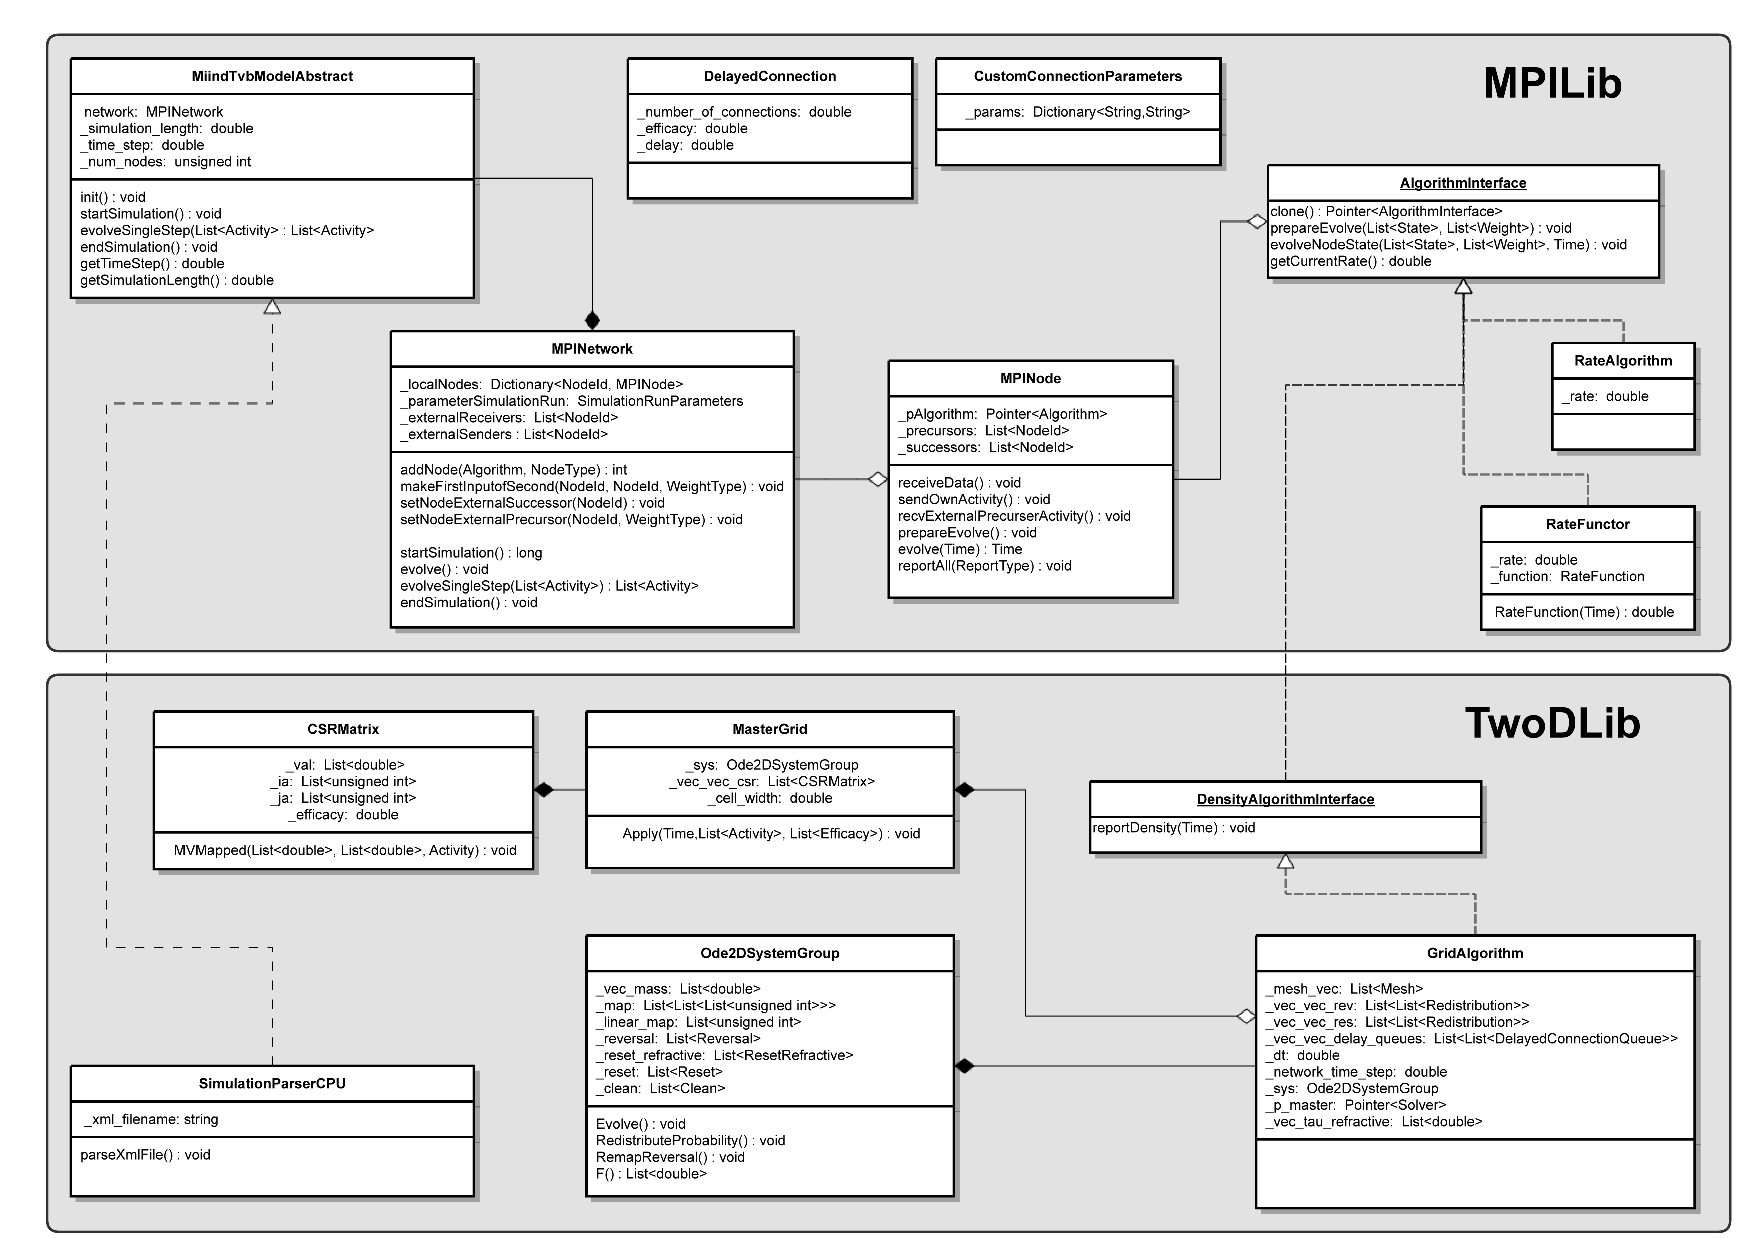
\includegraphics[width=\columnwidth]{images/miind_uml.pdf}
  \caption{A minimal UML diagram of MIIND. The two major libraries, MPILib and TwoDLib, are represented.}
  \label{fig:uml}
\end{figure}

\begin{figure}[!h]
  \centering
  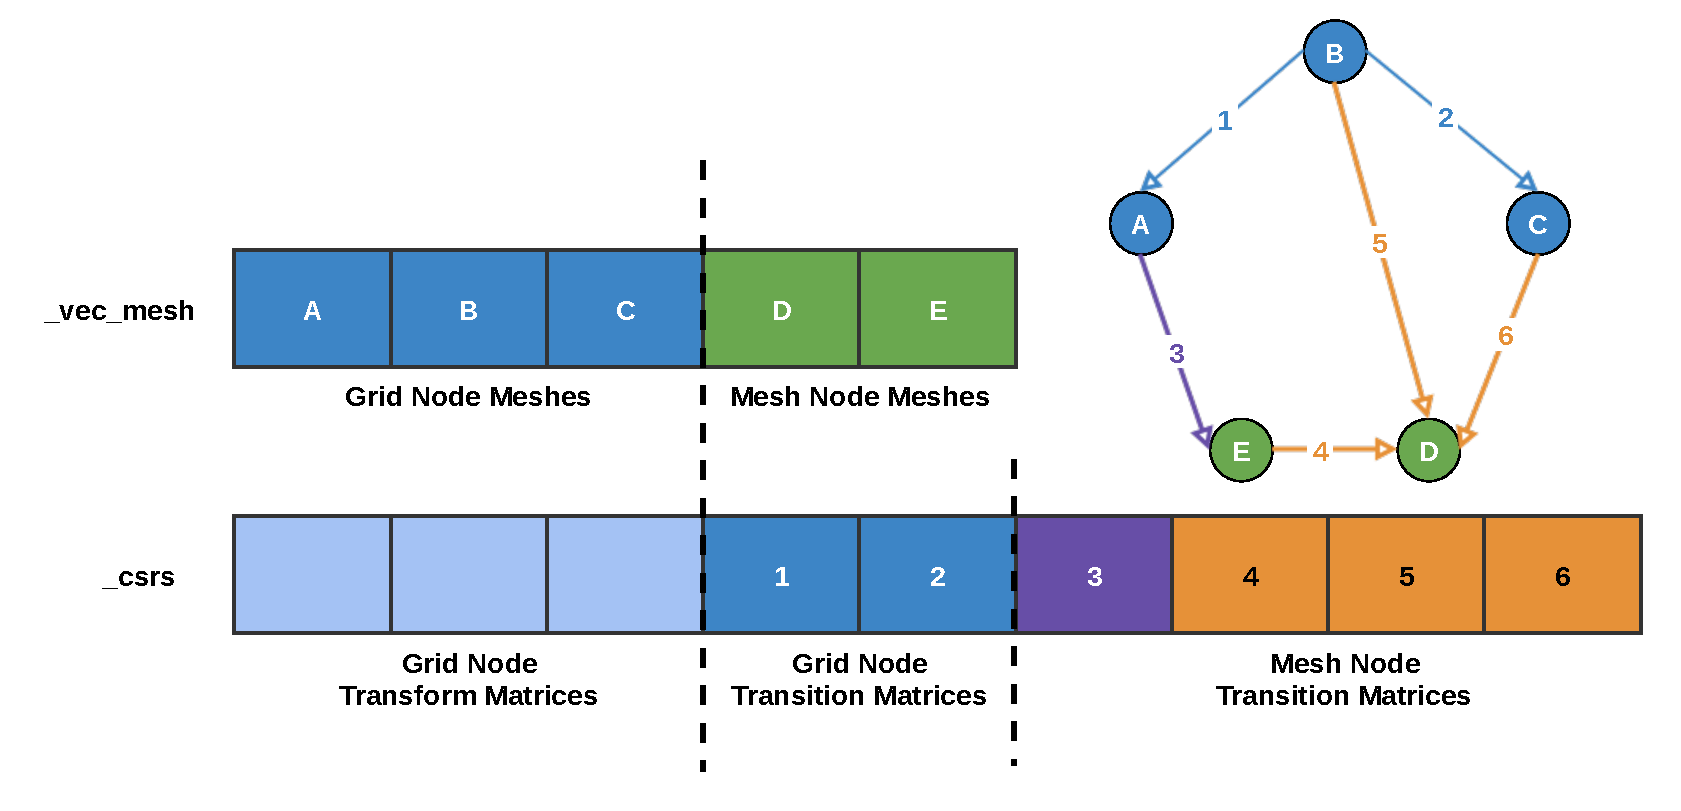
\includegraphics[width=\columnwidth]{images/neuroinformatics_structure.pdf}
  \caption{The data structures used for the vectorised form of MeshAlgorithm and GridAlgorithm. Nodes A, B, and C are GridAlgorithm nodes. Nodes D and E are MeshAlgorithm nodes. \_vec\_mesh holds the discretised probability density functions for the grid nodes and the mesh nodes. \_csrs holds the transition matrices which produce the deterministic dynamics of the grids and the matrices required to solve the Poisson master equation for each connection in the network. }
  \label{fig:cudastruct}
\end{figure}

\begin{figure}[!h]
  \centering
  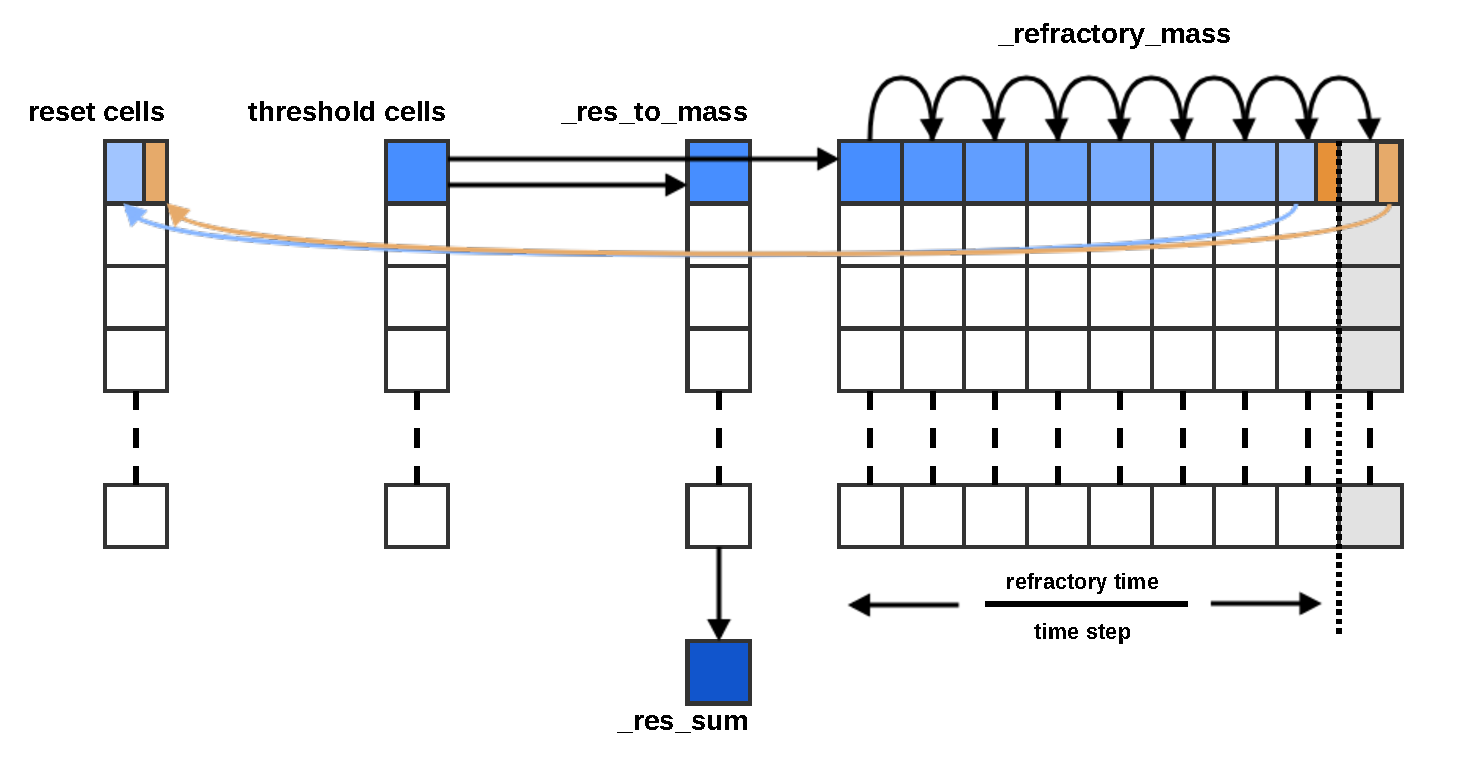
\includegraphics[width=\columnwidth]{images/neuroinformatics_reset.pdf}
  \caption{The vectorised implementation of reset functionality is very similar to that of the CPU version. However, there is an additional data structure, \_res\_to\_mass, which initially holds a copy of the mass in the threshold cells after each iteration. The structure is used to sum the cells in a parallel manner and the result is stored in \_res\_sum which can then be extracted from the GPU and used to calculate the average firing rate for each population.}
  \label{fig:cudareset}
\end{figure}

\begin{figure}[!h]
  \centering
  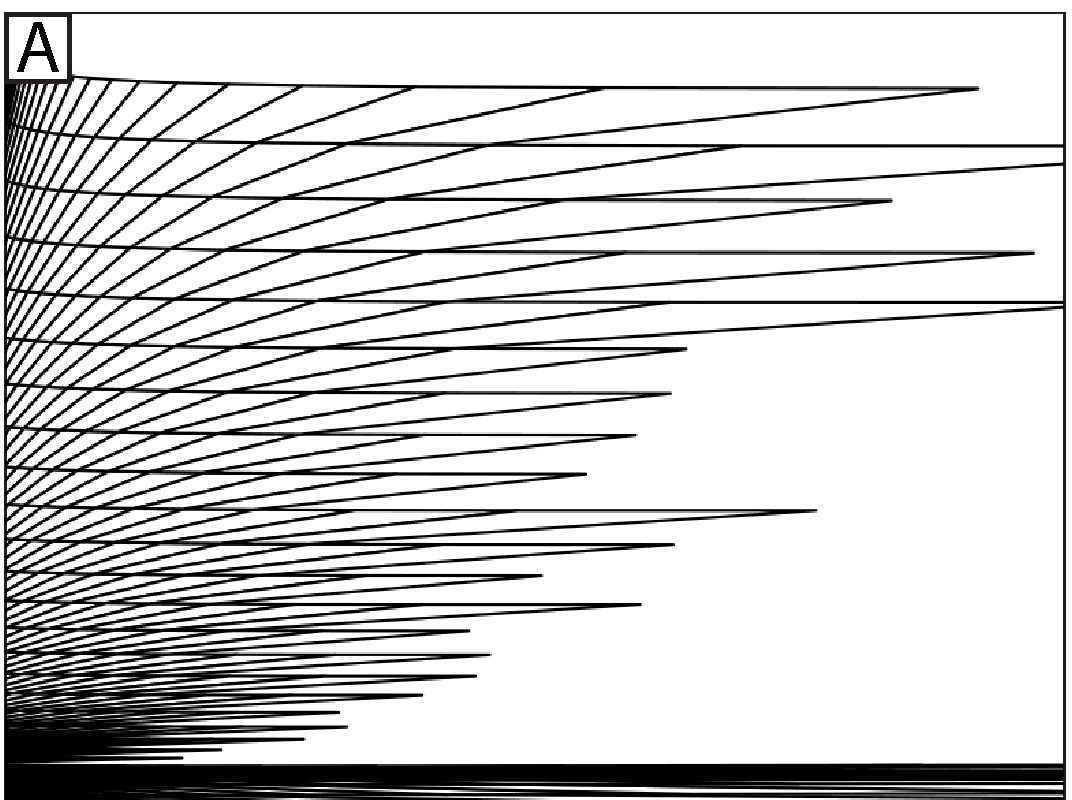
\includegraphics[width=0.49\columnwidth]{images/strip_tips_feathering3.pdf}
  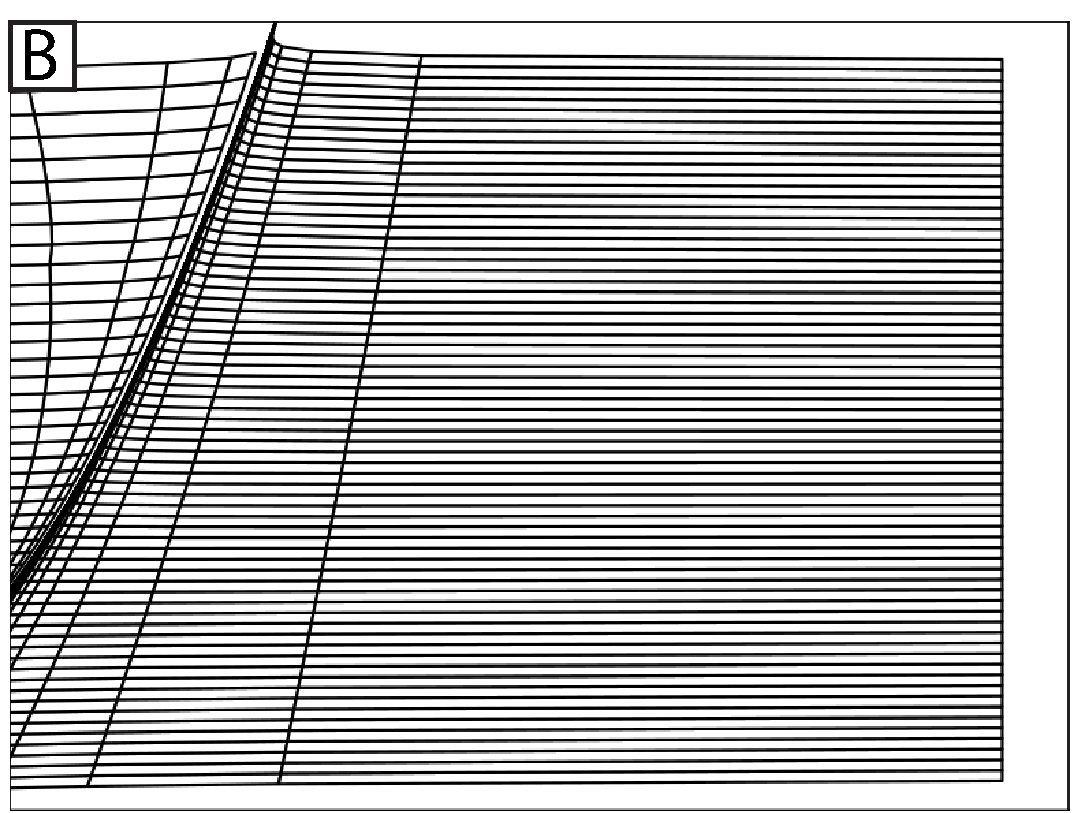
\includegraphics[width=0.49\columnwidth]{images/strip_tips_backwards2.pdf}
  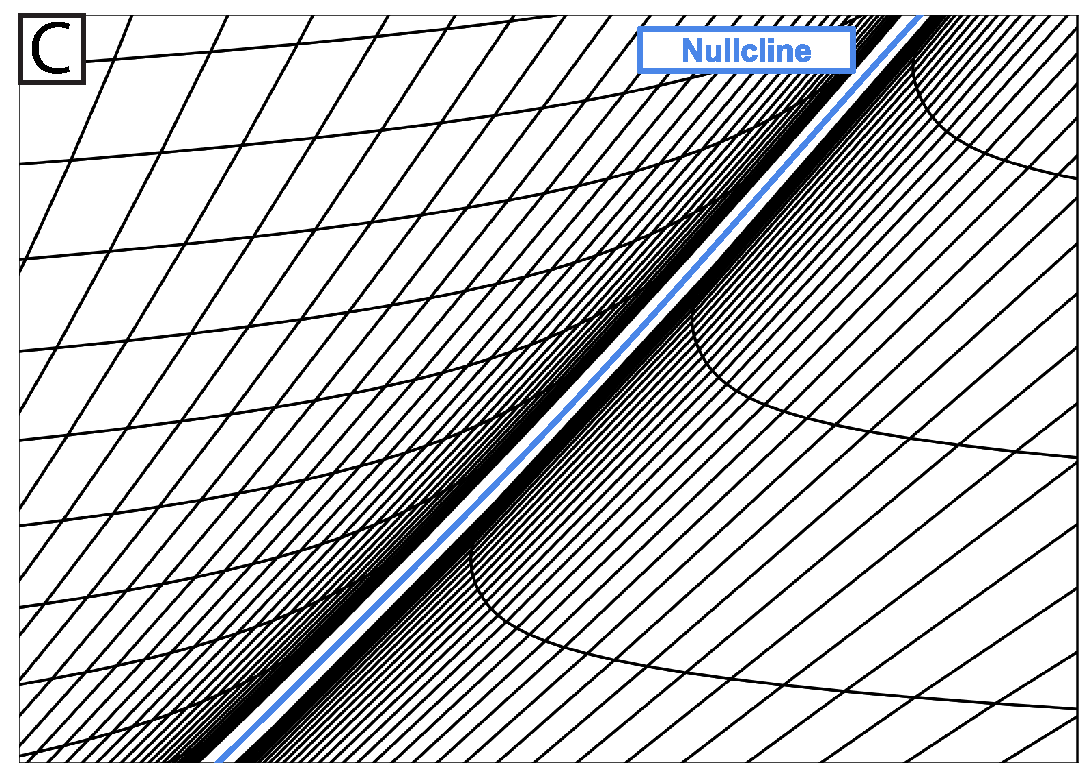
\includegraphics[width=0.49\columnwidth]{images/izh_nullcline_tips_strip.pdf}
  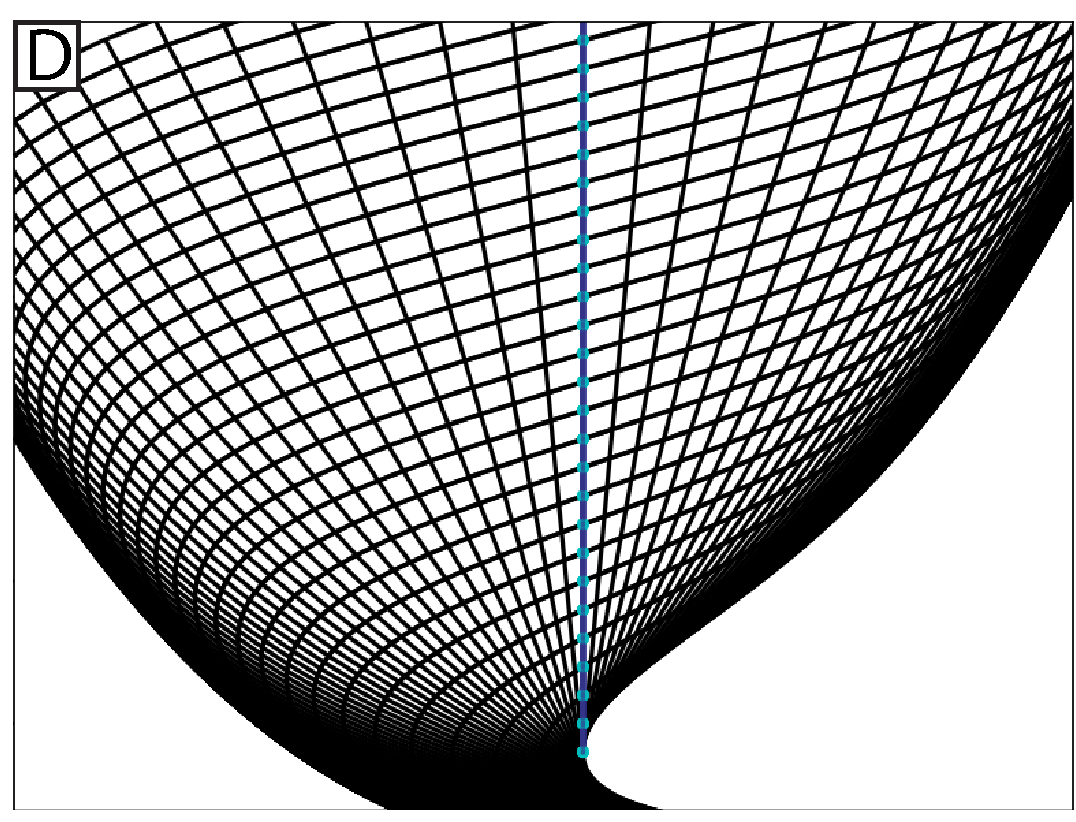
\includegraphics[width=0.49\columnwidth]{images/strip_stitch2.pdf}
  \caption{(A) As trajectories moving off to the right approach infinity, each strip is cut off at a different place producing a ``feathering'' effect which can make it difficult to identify threshold cells. (B) By picking starting points at a high value then backwards integrating, the feathering is eliminated. (C) Picking starting points for strip trajectories on either side of a nullcline and integrating away produces only a small gap where the nullcline itself lies. (D) An example of an area of low cell density split into two by a line of starting points (in blue). This technique handles the transition from high to low density cells on either side.}
  \label{fig:tips}
\end{figure}

%%% If you are submitting a figure with subfigures please combine these into one image file with part labels integrated.
%%% If you don't add the figures in the LaTeX files, please upload them when submitting the article.
%%% Frontiers will add the figures at the end of the provisional pdf automatically
%%% The use of LaTeX coding to draw Diagrams/Figures/Structures should be avoided. They should be external callouts including graphics.

\clearpage

\bibliographystyle{frontiersinSCNS_ENG_HUMS} %  for Science, Engineering and Humanities and Social Sciences articles, for Humanities and Social Sciences articles please include page numbers in the in-text citations
%\bibliographystyle{frontiersinHLTH&FPHY} % for Health and Physics articles
\bibliography{test}

\end{document}
